\section{Programming Model}

A question that one may pose is ``\emph{Why choose Fortran and not a
  more modern language like X for programming accelerator
  architectures?}''  The recent rise in interest in concurrency and
parallelism at the language level due to multicore CPUs and
many-core accelerators has driven a number of new language
developments, both as novel languages and extensions on existing ones.
However, for many scientific users with existing codes written in
Fortran, new languages and language extensions to use novel new
architectures present a challenge: how do programmers effectively use
them while avoiding rewriting code and potentially growing dependent
on a transient technology that will vanish tomorrow?  In this paper we
explore the constructs in Fortran that are particularly relevant to
GPU architectures.

In this section we present the Fortran subset employed in this paper.
This sub-setting language will allow scientific programmers to stay
within the Fortran language and yet have direct access to GPU
hardware.  We start by examining how this programming model relates to
developments in other languages.


\subsection{Comparison to Prior Fortran Work}



A number of previous efforts have exploited data-parallel programming
at the language level to utilize novel architectures.  The origin of
the array syntax adopted by Fortran in the 1990 standard can be found
in the APL language~\cite{iverson79apl}.  These additions to Fortran
allowed parallelism to be expressed with whole-array operations at the
expression level, instead of via parallelism within explicit DO-loops,
as implemented in earlier variants of the language (e.g., IVTRAN for the
Illiac IV).

The High Performance Fortran (HPF) extension of Fortran was proposed
to add features to the language that would enhance the ability of
compilers to emit fast parallel code for distributed and shared memory
parallel computers\cite{koelbel94hpf}.  One of the notable additions
to the language in HPF was syntax to specify the distribution of data
structures amongst a set of parallel processors.  HPF also introduced
an alternative looping construct to the traditional DO-loop called
{\tt FORALL} that was better suited for parallel compilation.  An
additional keyword, {\tt INDEPENDENT}, was added to allow the
programmer to indicate when the loop contained no loop-order
dependencies that allowed for parallel execution.  These constructs
are similar to {\tt DO CONCURRENT}, an addition to Fortran in 2008.

Interestingly, the parallelism features introduced in HPF did not
exploit the new array features introduced in 1990 in any significant
way, relying instead on explicit loop-based parallelism.  This
restriction allowed the language to support parallel programming that
wasn't easily mapped onto a pure data-parallel model.  The {\tt SHADOW}
directive introduced in HPF-2, and the {\tt HALO} in HPF+~\cite{benkner99hpf}
bear some similarity to the halo region concept that we discuss in this 
paper.

In some instances though, a purely data-parallel model is appropriate
for part or all of the major computations within a program.  One of
the systems where programmers relied heavily on higher level
operations instead of explicit looping constructs was the Thinking
Machines Connection Machine 5 (CM-5).  A common programming pattern
used on the CM-5 (that we exploit in this paper) was to write
whole-array operations from a global perspective in which computations
are expressed in terms of operations over the entire array instead of
a single local index.  The use of the array shift intrinsic functions
(like {\tt CSHIFT}) were used to build computations in which arrays
were combined by shifting the entire arrays instead of working on
local offsets based on single indices.  A simple 1D example is one in
which an element is replaced with the average of its own value and
that of its two direct neighbors.  Ignoring boundary indices that wrap
around, explicit indexing will result in a loop such as:

{\small
\begin{verbatim}
  do i = 2,(n-1)
    Xnew(i) = (X(i-1) + X(i) + X(i+1)) / 3
  end do
  PTR_SWAP(Xnew, X, tmp_ptr)
\end{verbatim}
}

\noindent In this loop, it is necessary to manually implement a double buffering scheme
in order to avoid mixing values computed in the current execution of the loop with values from a 
prior execution of the loop. When shifts are employed, this can be expressed as:

{\small
\begin{verbatim}
  X = (cshift(X,-1) + X + cshift(X,1)) / 3
\end{verbatim}
}

\noindent
The semantics of the shift intrinsic and operators like {\tt +}
applied to the whole array make it unnecessary to manually implement
the double buffering scheme found in the loop above.  Similar whole
array shifting was used in higher dimensions for finite difference
codes within the computational physics community for codes targeting
the CM-5 system.  Research in compilation of stencil-based codes that
use shift operators targeting these systems is related to the work
presented here~\cite{stencil-compiler}.

The whole-array model was attractive because it deferred
responsibility for optimally implementing the computations to the
compiler.  Instead of relying on a compiler to infer parallelism from
a set of explicit loops, the choice for how to implement loops was
left entirely up to the tool.

Unfortunately, this had two side effects that have limited broad
acceptance of the whole-array programming model in Fortran.  First,
programmers must translate their algorithms into a set of global
operations.  Finite difference stencils and similar computations are
traditionally defined in terms of offsets from some central index.
Shifting, while conceptually analogous, can be awkward to think about
for high dimensional stencils with many points.  Second, the semantics
of these operations are such that all elements of an array operation
are updated as if they were updated simultaneously.  In a program
where the programmer explicitly manages arrays and loops, double
buffering techniques and user managed temporaries are used to maintain
these semantics.  Limited attention to optimizing memory usage due to
this intermediate storage by compilers has led to these constructs
seeing little adoption by programmers.

%When the compiler is responsible for managing this
%intermediate storage, it has historically proven that they are
%inefficient and generate code that requires far more temporary storage
%than really necessary.  
%This is not a flaw of the language constructs,
%but a sign of the lack of sophistication of the compilers with respect
%to their internal analysis to determine how to optimally generate this
%intermediate storage.

An interesting line of language research that grew out of HPF was that
associated with the ZPL language at the University of
Washington~\cite{chamberlain04zpl} and Chapel, an HPCS language developed by
Cray~\cite{chamberlainchapel}.  In ZPL, programmers adopt a similar global view
of computation over arrays, but define their computations based on regions,
which provide a local view of the set of indices that participate in the update
of each element of an array.  A similar line of research in the functional
language community has investigated array abstractions for expressing
whole-array operations in the Haskell language in the REPA (regular, shape-polymorphic,
parallel array) library~\cite{keller10repa}.

\subsection{Fortran Language Subset}

The static analysis and source-to-source transformations used in this work
require the programmer to use a language subset that employs a data-parallel
programming model.  In particular, it encourages the use of array notation,
pure elemental functions, and pure procedures.  From these language constructs, we
are able to easily transform Fortran procedures to a lower-level OpenCL kernel
implementation.

\subsubsection*{Array notation}

Fortran has a rich array syntax that allows programmers to write statements in
terms of whole arrays or subarrays, with data-parallel operators to compute on
the arrays.  Array variables can be used in expressions based on whole-array
operations.  For example, if {\tt A}, {\tt B}, and {\tt C} are all arrays of the
same rank and shape and {\tt s} is a scalar, then the statement

{\small
\begin{verbatim}
 C = A + s*B
\end{verbatim}
}

\noindent
results in the element-wise sum of {\tt A} and the product of {\tt s} times the
elements of {\tt B} being stored in the corresponding elements of {\tt C}. The
first element of {\tt C} will contain the value of the first element of {\tt A}
added to the first element of {\tt c*B}.  Note that no explicit iteration over
array indices is needed and that the individual operators, plus, times, and
assignment are applied by the compiler to individual elements of the arrays
independently.  Thus the compiler is able to spread the computation in the
example across any hardware threads under its control.

\subsubsection*{Pure elemental functions}

An elemental function consumes and produces scalar values, but can be applied to
variables of array type such that the function is applied to each and every
element of the array.  This allows programmers to avoid explicit looping and
instead simply state that they intend a function to be applied to every element
of an array in parallel, deferring the choice of implementation technique to the
compiler.  Pure elemental functions are intended to be used for data-parallel
programming, and as a result must be side effect free and mandate an {\tt
intent(in)} attribute for all arguments. 

For example, the basic array operation shown above could be refactored into a pure
elemental function,

{\small
\begin{verbatim}
  pure elemental real function foo(a, b, s)
    real, intent(in) :: a, b, s
    foo = a + s*b
  end function
\end{verbatim}
}

\noindent and called with

{\small
\begin{verbatim}
  C = foo(A, B, s)
\end{verbatim}
}

Note that while {\tt foo} is defined in terms of purely scalar quantities, it
can be \emph{applied} to arrays as shown.  While this may seem like a trivial
example, such simple functions may be composed with other elemental functions to
perform powerful computations, especially when applied to arrays.  Our prototype
tool transforms pure elemental functions to inline OpenCL functions.  Thus there is
no penalty for usage of pure elemental functions and they provide a convenient
mechanism to express algorithms in simpler segments.

It should be noted that in Fortran 2008,
the concept of impure elemental functions was introduced.  This requires that
elemental functions now need to be explicitly labeled as pure to indicate that they
are side effect free.

\subsubsection*{Pure procedures}

Pure procedures, like pure elemental functions, must be free of side effects.  Unlike
pure elemental functions that require arguments to have an {\tt intent(in)}
attribute, they may change the contents of array arguments that are passed to
them.  The absence of side effects removes ordering constraints that could
restrict the freedom of the compiler to invoke pure functions out of order and
possibly in parallel.  Procedures and functions of this sort are also common in
pure functional languages like Haskell, and are exploited by compilers in order
to emit parallel code automatically due to their suitability for compiler-level
analysis.

Since pure procedures don't have side effects they are candidates for running on
accelerators in OpenCL.  Currently our prototype tool only transforms pure procedures
to OpenCL kernels that \emph{do not} call other procedures, except for pure elemental
functions, either defined by the user or intrinsic to Fortran.

\subsection{New Procedures}

Borrowing ideas from ZPL, we introduce a concept of a region to Fortran with a
set of functions that allow programmers to work with subarrays in expressions.
In Fortran, these functions return a copy of or a pointer to an existing array or array section.
This is unlike ZPL, where regions are analogous to index sets and are used
primarily for address resolution within an array without dictating storage
related behavior.  The functions that we propose are similar in that they allow
a programmer to deal with index regions that are meaningful to their algorithm,
and automatically induce a halo (or ghost) cell pattern as needed in the
implementation generated by the compiler, where the size of an array is
implicitly increased to provide extra array elements surrounding the interior 
portion of the array.  It is important to note, however, that all memory allocated
by the programmer must explicitly contain the extra array elements in the halo.
%%%This is critical to reducing the amount of code that the programmer is forced to write, as the halo cells are often where boundary errors and off-by-one errors may occur in code that is manually generated.

Region functions are similar to the shift operator as they can be used
to reference portions of the array that are shifted with respect to
the interior portion.  However, unlike the shift operator, regions are
not expressed in terms of boundary conditions and thus don't
explicitly \emph{require} a knowledge of, nor the application of,
boundary conditions locally (global boundary conditions must be
explicitly provided by the programmer outside of calls to kernel
procedures).  Thus, as will be shown below, regions are more suitable
for usage by OpenCL thread groups which access only local subsections
of an array stored in global memory.

\begin{figure}[!t]
\centering
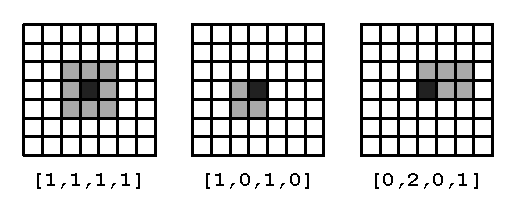
\includegraphics[width=2.5in]{halo.pdf}
\caption{An illustration of three simple halo regions around a single central
index.}
\label{fig:halos}
\end{figure}

ForOpenCL provides two new functions that are defined in Fortran and are used
in array-syntax operations.  Each function takes an integer array halo argument
that specifies the number of ghost cells on either side of a region, for each
dimension.  For example {\tt halo = [left, right, down, up]} specifies a halo
for a two-dimensional region.  Example halo regions are illustrated in
Figure~\ref{fig:halos}.  These functions are:

\begin{itemize}

\item {\tt region\_cpy(array, halo)}: a pure function that returns a copy of
  the interior portion of the array specified by halo.

\item {\tt region\_ptr(array, halo)}: an impure function that returns a pointer 
  to the portion of the array specified by halo.

\end{itemize}

It should be noted that the function {\tt region\_cpy} is pure and thus can be
called from within a pure kernel procedure, and {\tt
region\_ptr} is impure because it aliases the array parameter.  However as will
be shown below, the usage of {\tt region\_ptr} is constrained so that it does not
introduce side effects in the functions that call it.  These two functions are
part of the language recognized by the compiler and though {\tt region\_cpy}
returns a copy of a portion of an array \emph{semantically}, the compiler is not
forced to actually make a copy and is free to enforce copy semantics through
other means.  In addition to these two new functions, ForOpenCL provides the
compiler directive, {\tt \!\$OFP PURE, KERNEL}, which specifies that a pure subroutine
can be transformed to an OpenCL kernel and that the subroutine is pure
except for calls to {\tt region\_ptr}.  These directives are not strictly
necessary for the technique described in this paper, but aid in automated
identification of specific kernels to be transformed to OpenCL.  A directive-free
implementation would require the transformation tool be provided the set of 
kernels to work via a user defined list.

\subsection{Advantages}

There are several advantages to this style of programming using array
syntax, regions, and pure and elemental functions:

\begin{itemize}
\item There are no loops or index variables to keep track of.  Off by
  one index errors and improper handling of array boundaries are a
  common programming mistake.
\item The written code is closer to the algorithm, easier to
  understand, and is usually substantially shorter.
\item Semantically the intrinsic function {\tt region\_cpy} returns an array by value.
  This is usually what the algorithm requires.
\item Pure elemental functions are free from side effects, so it is
  easier for a compiler to schedule the work to be done in parallel.
\end{itemize}

Data parallelism has been called collection-oriented programming by
Blelloch~\cite{blelloch90}.  As the {\tt cshift} function and the array-valued
expressions all semantically return a value, this style of programming is also
similar to functional programming (or value-oriented programming).  It should be
noted that the sub-setting language we employ goes beyond pure data parallelism
by the use of pure (other than calls to {\tt region\_ptr}) subroutines and
not just elemental functions.

Unfortunately, this style of programming has never really caught on because when
array syntax was first introduced in Fortran, performance of codes using these features was
relatively poor and thus programmers shied away from using array syntax (even
recently, some are actively counseling against its usage because of performance
issues~\cite{Levesque:SC08}).  Thus the Fortran community was caught in a
classic ``chicken-and-egg'' conundrum: (1) programmers didn't use it because it
was slow; and (2) compilers vendors didn't improve it because programmers didn't
use it.  A goal of this paper is to demonstrate that parallel programs written
in this style of Fortran can achieve good performance on accelerator architectures.

\subsection{Restrictions}

Only pure Fortran procedures are transformed into OpenCL kernels.  This restriction
is lifted slightly to allow calls to {\tt region\_ptr} from within a kernel procedure.  The
programmer must explicitly call these kernels using Fortran interfaces in the ForOpenCL
library (described below).  It is also possible, using ROSE, to modify the calling
site so that the entire program can be transformed, but this functionality is
outside the scope of this paper.  Here we specifically examine transforming
Fortran procedures to OpenCL kernels.  Because OpenCL support is relatively new
to ROSE, some generated code must be modified.  For example, the {\tt
  \_\_global} attribute for kernel arguments was added by hand.

It is assumed that memory for all arrays reside on the device.  The programmer
must copy memory to and from the device.  In addition, array size (neglecting
ghost cell regions) must be multiples of the global OpenCL kernel size.

Array variables within a kernel procedure (specified by the {\tt \!\$OFP PURE,
  KERNEL} directive) must be declared as contiguous.  A kernel procedure may not
call other procedures except for limited intrinsic functions (primarily math),
user-defined elemental functions, and the {\tt region\_cpy} and {\tt region\_ptr}
functions.  Future work will address non-contiguous arrays (such as those that
result from strided access) by mapping array strides to gather/scatter-style
memory accessors.

Array parameters to a kernel procedure must be declared as either intent(in) or
intent(out); they cannot be intent(inout).  A thread may read from an extended
region about its local element (using the {\tt region\_cpy} function), but can
only write to the single array element it owns.  If a variable were intent(inout),
a thread could update its array element before another thread had read from that
element.  This restriction requires double buffering techniques.
